\documentclass[11pt,a4paper]{article}
\usepackage[utf8]{inputenc}
\usepackage[T1]{fontenc}
\usepackage{lmodern}
\usepackage[margin=2.5cm]{geometry}
\usepackage{xcolor}
\usepackage{amsmath}
\usepackage{hyperref}
\usepackage{booktabs}
\usepackage{longtable}
\usepackage{enumitem}
\usepackage{parskip}
\usepackage{listings}
\usepackage{tikz}
\usetikzlibrary{shapes.geometric,arrows.meta,positioning,fit,backgrounds,calc}

\hypersetup{colorlinks=true, linkcolor=blue!60!black, urlcolor=blue!60!black,
            citecolor=blue!60!black}

\definecolor{codebg}{HTML}{F5F5F5}
\definecolor{codekw}{HTML}{0033B3}
\definecolor{codecm}{HTML}{8E908C}
\lstset{
  basicstyle=\ttfamily\footnotesize,
  backgroundcolor=\color{codebg},
  keywordstyle=\color{codekw}\bfseries,
  commentstyle=\color{codecm}\itshape,
  language=C++,
  breaklines=true,
  showstringspaces=false,
  frame=single,
  framerule=0pt,
  xleftmargin=4pt,
  xrightmargin=4pt,
  aboveskip=6pt,
  belowskip=6pt,
}

\title{MIPster Cut and Heuristic Orchestration}
\author{MIPster Development Team}
\date{June 2026}

\begin{document}
\maketitle
\tableofcontents
\newpage

\section{Overview}

MIPster (a Cbc fork) drives a branch--and--cut search.  At every node
--- including the root --- it alternates three things in a fixed
sequence: \textbf{(1)} solve / re-solve the LP relaxation,
\textbf{(2)} run a battery of cut generators in batch and apply the
selected cuts, \textbf{(3)} optionally run primal heuristics on the
fractional solution.  This document explains, with file/line
pointers into \texttt{src/}, how that orchestration is implemented:
how each pass decides whether to keep generating cuts (the
``\texttt{ifMove}'' / diminishing--returns logic), how individual
generators are throttled across passes, the parallel-cuts execution
mode, the global cut pool, and the mechanisms that rank cuts when
too many are produced.

The two source files driving this are:
\begin{itemize}[leftmargin=*]
  \item \texttt{src/CbcModel.cpp} --- per-pass orchestration
        (\texttt{solveWithCuts}), per-generator post-loop adjustment,
        \texttt{serialCuts}, \texttt{takeOffCuts}, and
        \texttt{doHeuristicsAtRoot}.
  \item \texttt{src/CbcThread.cpp} --- \texttt{parallelCuts}.
\end{itemize}

\section{Root vs. tree control loop}
\label{sec:rootloop}

\subsection*{High level}

\texttt{CbcModel::branchAndBound} (around \texttt{CbcModel.cpp:2700})
performs the root work in this order:

\begin{enumerate}[leftmargin=*]
  \item Initial LP solve and presolve setup.
  \item \textbf{Pre-cut heuristics:} \texttt{doHeuristicsAtRoot()} at
        \texttt{CbcModel.cpp:3056} (FPump, dive conflict harvest, etc.).
  \item \textbf{Root cut loop:}
        \texttt{solveWithCuts(cuts, maximumCutPassesAtRoot\_, NULL)}
        at \texttt{CbcModel.cpp:3386} --- up to
        \texttt{maximumCutPassesAtRoot\_} passes of \emph{(generate
        cuts $\to$ apply $\to$ resolve $\to$ post-pass heuristics)}.
  \item \textbf{Per-generator adjustment:} after the loop, every cut
        generator's \texttt{howOften} is updated based on how much it
        contributed at the root (\texttt{CbcModel.cpp:10080--10591}).
  \item Branch-and-bound proper begins; at every node
        \texttt{solveWithCuts(cuts, maximumCutPasses\_, node)} is
        called from \texttt{CbcModel.cpp:17919}.
\end{enumerate}

\subsection*{The pass loop in \texttt{solveWithCuts}}

\texttt{solveWithCuts} (\texttt{CbcModel.cpp:8333+}) is the same
routine used at root and at every node; the second argument
(\texttt{numberTries}) gates how many passes are allowed.  The
loop body lives at \texttt{CbcModel.cpp:9000--9711}.  Each pass:

\begin{enumerate}[leftmargin=*]
  \item Increments \texttt{currentPassNumber\_} (line~9001).
  \item On the very first pass, scans the global cut pool
        \texttt{globalCuts\_} for cuts violated by the current
        relaxation (line~9066) and selects up to a budget by
        \emph{violation-sorted} order (see \S\ref{sec:cutpool} for
        the pool itself and \S\ref{sec:globalpool-budget} for how
        the element budget is computed).
  \item Calls either \texttt{serialCuts} or \texttt{parallelCuts}
        (lines~9272--9279) to invoke every active generator.
  \item Skips a primal-heuristic block on pass~1 of the root, runs
        it on later passes (line~9295).
  \item Applies the chosen cuts via
        \texttt{solver\_->applyRowCuts(\dots)} (line~9514).
  \item Re-solves the LP via \texttt{resolve(\dots)} (line~9533).
  \item Calls \texttt{takeOffCuts} (line~9582) to drop cuts that
        slacken (\S\ref{sec:takeoff}).
  \item Applies the diminishing-returns / \texttt{ifMove} test
        (lines~9595--9711) and decides whether to keep looping
        (see \S\ref{sec:ifmove} for the full criterion).
\end{enumerate}

So the answer to ``do we add X, reoptimize and then run Y?'' is:
\textbf{all generators run together in one batch per pass, then one
resolve, then heuristics}, then back to step 3.  Generators are not
interleaved one-at-a-time with re-solves.

\subsection*{Tree-depth gating}
\label{sec:treedepth}

Inside the tree, \texttt{solveWithCuts} additionally honours
\texttt{treeCutDepth\_} (\texttt{CbcModel.cpp:8357--8378}): below the
threshold \texttt{numberTries=1} (cuts are tried), above it
\texttt{numberTries=0} (only resolve).  The deeper helper
\texttt{doCutsNow} at \texttt{CbcModel.cpp:18885--18942} provides a
finer per-depth gate used by individual generators (see
\S\ref{sec:docutsnow}).

\subsection*{\texttt{doCutsNow} per-depth gate}
\label{sec:docutsnow}

\texttt{CbcModel::doCutsNow(int allowForTopOfTree) const}
(\texttt{CbcModel.cpp:18885--18942}) returns \texttt{true} when the
current node depth and the configured \texttt{whenCuts\_} mode agree
that cuts should be generated here.  The author's comment at
\texttt{CbcModel.cpp:18880--18883} states the four argument values:

\begin{itemize}[leftmargin=*]
  \item \texttt{0} --- only on multiples of the configured depth.
  \item \texttt{1} --- also allow ``at top of tree''
        (\texttt{currentDepth\_ <= shallow}).
  \item \texttt{2} --- ``cuts allowed anywhere apart from root''.
  \item \texttt{3} --- ``smallest valid depth $>$ shallow''; in the
        currently-active \texttt{TRY\_IDEA1=2} branch this collapses
        to ``only at exactly depth~10''
        (\texttt{CbcModel.cpp:18934--18936}).
\end{itemize}

Internally, \texttt{whenCuts\_} (set via \texttt{setWhenCuts},
exposed on the CLI as \texttt{-cuts}) is decoded into a
\texttt{top}/\texttt{shallow}/\texttt{when} triple
(\texttt{CbcModel.cpp:18914--18916}); for small models
($\le 500$ rows$+$cols) and \texttt{whenCutsUse $<$ 0} the routine
falls into a simpler depth-parity branch
(lines~18899--18911).  This is the single place where per-generator
\texttt{depthCutGenerator\_} settings (\S\ref{sec:howoften}) and the
tree-wide \texttt{treeCutDepth\_} (\S\ref{sec:treedepth}) interact
with node depth.

\section{The diminishing-returns / \texttt{ifMove} logic}
\label{sec:ifmove}

The cut loop terminates early if cuts stop helping the LP bound.
The relevant code is at \texttt{CbcModel.cpp:9595--9711}, and is
controlled by \texttt{minimumDrop\_} (default \texttt{1.0e-7}, set in
\texttt{CbcModel.cpp:6001/6191}; tightened in
\texttt{CbcSolver.cpp} to
\texttt{min(5e-2,\,|obj|*1e-5+1e-5)}).

\subsection*{The rolling history}

A buffer keeps the last \texttt{CUT\_HISTORY=7} pass objectives
(\texttt{CbcModel.cpp:8381}).  Two flags steer the test:

\begin{lstlisting}
int  experimentBreak = (moreSpecialOptions_ >> 11) & 3;   // 9969
bool increaseDrop    = (moreSpecialOptions_ & 8192) != 0; // 9971
\end{lstlisting}

\subsection*{The badObj / goodDrop test}

After the resolve, the loop compares the new bound against the
oldest one in the history window:

\begin{lstlisting}
bool badObj  = thisObj < cut_obj[CUT_HISTORY-1] + minimumDrop_;
double goodDrop = thisObj - cut_obj[0];
// nBadPasses incremented if drop is too small
if (badObj && allowEarlyTermination && !keepGoing)
  numberTries = 0;          // exit the loop
\end{lstlisting}

The loop is allowed to exit when:
\begin{itemize}[leftmargin=*]
  \item \texttt{badObj} fires (no progress vs.\ the 7-pass window),
        \emph{and}
  \item no generator flagged itself as ``must call again''
        (\texttt{keepGoing}), \emph{and}
  \item the early-termination guard is on
        (\texttt{allowEarlyTermination}).
\end{itemize}

If \texttt{increaseDrop} is set, \texttt{minimumDrop\_} ramps up over
passes, making the loop bail out faster.  \texttt{experimentBreak}
toggles two stricter variants of the test (used for tuning runs).

\subsection*{Per-pass ``ifMove'' for individual cuts}

Beyond the loop-level test, individual cuts can be marked
``\texttt{ifMove}'' through their generator's mode.  This translates
into an effectiveness threshold passed to \texttt{takeOffCuts}: cuts
whose effectiveness is below the threshold and whose row is basic in
the current basis are dropped (\S\ref{sec:takeoff}).  In other
words, ``ifMove'' = ``keep the cut only if it is still binding /
effective after the resolve.''

\section{Per-generator throttling}
\label{sec:howoften}

Each \texttt{CbcCutGenerator} carries:
\begin{itemize}[leftmargin=*]
  \item \texttt{whenCutGenerator\_} (a.k.a.\ \emph{howOften}):
        $0$ = off, $1$ = every pass, $-1$ = root only,
        $-99$ = ``almost off (only when the search is desperate)'',
        $-100$ = permanently off.
  \item \texttt{depthCutGenerator\_}: depth multiplier
        (run only when $depth \bmod n=0$).
  \item \texttt{switchOffIfLessThan\_}: yield threshold below which
        the generator is shut off post-root.
  \item A \texttt{switches\_} bitfield with 16 flags, including
        \texttt{normal}, \texttt{atSolution}, \texttt{whenInfeasible},
        \texttt{mustCallAgain}, \texttt{switchedOff},
        \texttt{ineffectualCuts}, \texttt{whetherToUse},
        \texttt{whetherInMustCallAgainMode},
        \texttt{whetherCallAtEnd}, \texttt{needsRefresh},
        \texttt{cleanLagrangean}.  Definitions in
        \texttt{src/CbcCutGenerator.hpp} (lines covering the bit
        constants).
\end{itemize}

The per-call gate is \texttt{CbcCutGenerator::generateCuts}
(\texttt{src/CbcCutGenerator.cpp:186--262}).  Simplified:

\begin{lstlisting}
int howOften = whenCutGenerator_;
if (howOften <= -100 || howOften == 0) return false;     // off
int pass = model_->getCurrentPassNumber() - 1;
bool doThis = (model_->getNodeCount() % howOften) == 0;
if (depthCutGenerator_ > 0)
  doThis = (currentDepth % depthCutGenerator_) == 0;
if (whenCutGeneratorInSub_ == -200 && model_->parentModel())
  doThis = false;                                        // off in subtree
\end{lstlisting}

Once cuts are produced, the per-call exit also flips the generator's
\texttt{ineffectualCuts} bit if no cut was retained --- this feeds
the post-loop adjustment described next.

\subsection*{Post-loop \texttt{howOften} decay (root only)}

After the root cut loop, \texttt{CbcModel.cpp:10080--10591} loops
over the generators and rewrites \texttt{howOften} based on how much
they actually contributed.  Highlights:

\begin{lstlisting}
// 10140 -- if no objective change and rows grew >20%
if (numberRowsAtContinuous_ * 1.2 < numberRowsAtStart
    && noObjectiveChange)
  willBeCutsInTree = -1;

// 10419 -- generator-specific shut off
if (howOften == -98 && switchOffIfLessThan > 0
    && objImprovement < 0.005 * fabs(startObj) + 1e-5)
  howOften = -99;

// 10474..10534 -- rebuild howOften from cut yield
//   no cuts        -> howOften = -99 (almost off)
//   few cuts       -> howOften = max(2, ...)
//   many cuts      -> howOften = 1 (every pass)

// 10578
generator_[i]->setHowOften(howOften);
\end{lstlisting}

The ``\texttt{ifMove}'' parameter style (\texttt{-cuts ifmove},
\texttt{-gomory ifmove}, etc.) ultimately sets \texttt{howOften} to
$-98$ for the corresponding generator, which causes the
\texttt{switchOffIfLessThan\_} test above to demote it to $-99$
unless it pulled its weight at the root.

\textbf{Important interaction with pass-0 early disable.}
Generators with \texttt{switchOffIfLessThan\_ > 0} are also disabled
\emph{during} root cutting: at the end of pass~0
(\texttt{CbcCutGenerator.cpp:1583--1591}), if the generator produced
fewer row cuts than the threshold, \texttt{whenCutGenerator\_} is set
directly to $-100$.  The post-loop then reads \texttt{howOften =
-100} at the start of its per-generator iteration, skips the
adjustment logic, and \emph{only emits a \texttt{CBC\_GENERATOR}
summary message if the generator found at least one cut overall}.
This means TwoMirCuts (\texttt{switchOffIfLessThan = 1}) and
ZeroHalf (\texttt{switchOffIfLessThan = 2}) may be silently absent
from the cut summary on problems where they find nothing --- even
though they were configured and ran on pass~0.  The fix applied in
MIPster removes the ``$n > 0$'' guard so all generators are always
reported at root (\texttt{CbcModel.cpp:10757--10774}).

\subsection*{Generator scan caps}

Two compile-time caps live in \texttt{src/CbcCutGenerator.hpp}:

\begin{lstlisting}
#define SCANCUTS         1000
#define SCANCUTS_PROBING 1000
\end{lstlisting}

These bound the number of rows / columns a generator scans per call
(generators that respect them stop early on huge models).

\section{Serial vs.\ parallel cuts}
\label{sec:parallel}

Two paths exist for invoking the generators in a pass.

\subsection*{\texttt{serialCuts} (default)}

\texttt{CbcModel::serialCuts} (\texttt{CbcModel.cpp:10797--10915})
walks \texttt{generator\_[0\,..\,numberCutGenerators\_-1]} in a
single thread, calling \texttt{generateCuts} on each one that is
\texttt{normal()}, not \texttt{switchedOff()}, satisfies its
\texttt{needsOptimalBasis()} requirement, and matches the current
\texttt{whetherCallAtEnd()} phase.  Cuts produced are merged into
the local \texttt{theseCuts} pool.

\subsection*{\texttt{parallelCuts}}

\texttt{CbcModel::parallelCuts} (\texttt{src/CbcThread.cpp:1954})
runs each generator in its own thread via
\texttt{master->waitForThreadsInCuts(\dots)}, then merges the
results.  It honours \texttt{mustCallAgain} (sets the loop's status
to ``keep going'').

The selection happens at \texttt{CbcModel.cpp:9272--9279}:

\begin{lstlisting}
if ((threadMode_ & 2) == 0 || numberNodes_)
  serialCuts(theseCuts, node, fullScan, eachCutLimit);
else
  parallelCuts(master_, theseCuts, node, eachCutLimit);
\end{lstlisting}

So parallel cuts are used \emph{only at the root} (\texttt{numberNodes\_==0})
and only when bit~2 of \texttt{threadMode\_} is set.  Inside the
tree, threading is used for parallel \emph{node} expansion (bit~1)
and parallel heuristics (bit~4) instead.

\section{Global cut pool and ranking}
\label{sec:cutpool}

\subsection*{Yes, it is a global pool}

There is exactly one cut pool per \texttt{CbcModel}, declared at
\texttt{CbcModel.hpp:3028}:

\begin{lstlisting}
CbcRowCuts globalCuts_;
\end{lstlisting}

It is ``global'' in the sense that \emph{any} node can deposit cuts
into it and \emph{every} subsequent node may pick them up via the
pass-1 re-scan in \texttt{solveWithCuts}
(\texttt{CbcModel.cpp:9066--9131}).  Cuts placed here must therefore
be \textbf{globally valid} --- valid for the whole MIP, not just the
sub-problem at one node.  Generators (and \texttt{takeOffCuts})
mark cuts globally valid via
\texttt{OsiRowCut::setGloballyValid()} or
\texttt{setGloballyValidAsInteger(2)} before insertion (e.g.\
\texttt{CbcModel.cpp:3336, 3584, 4893--4905, 8509, 9042, 9802}).

\subsection*{Internal structure: hash-deduplicated array}

\texttt{CbcRowCuts} (\texttt{src/CbcCountRowCut.cpp:383--660}) is a
dynamic array of \texttt{OsiRowCut2 *} (\texttt{rowCut\_[]}) backed
by a separately-chained hash table (\texttt{hash\_[]}, sized
\texttt{hashMultiplier\_ * size\_}).  The flow inside
\texttt{addCutIfNotDuplicate} (line 587) is:

\begin{enumerate}[leftmargin=*]
  \item If the array is at capacity, double it
        (\texttt{size\_ = 2 * size\_ + 100} at line 595) and
        rebuild the hash table from scratch.  So the pool is in
        practice unbounded; ``hash full'' only happens transiently
        during the rebuild and is handled by widening the cut's
        bounds rather than dropping it (\texttt{lines 626--635}).
  \item Compute the cut's hash (\texttt{hashCut(cut, hashSize)}) ---
        a function of the sorted index/coefficient pattern.
  \item Walk the chain at that bucket; if a cut with the same
        \texttt{same(cutA, cutB)} signature is found,
        return $1$ (``not added, duplicate'').
  \item Otherwise sort the cut's indices, sanity-check coefficient
        magnitudes ($10^{-12} \le |a_i| \le 10^{12}$), append it to
        \texttt{rowCut\_} and link it into the hash chain.  Return $0$.
  \item Return value $-1$ is reserved for ``no space'' and is never
        actually returned in practice (the auto-resize covers it).
\end{enumerate}

So the pool is effectively a \textbf{hash-set of globally valid row
cuts with insertion-order preservation}.  Lookup is O(1)~average,
insertion is O(1)~amortised, and there is no built-in eviction
policy beyond manual \texttt{truncate(n)} (line 524) and
\texttt{eraseRowCut(seq)} (line 465).  See
\S\ref{sec:cutpool-vs-coincutpool} for how this differs from the
ranking-aware \texttt{CoinCutPool} used inside individual cut
generators.

\subsection*{Who deposits into the pool}

Cuts arrive in \texttt{globalCuts\_} from many places --- it is the
solver's persistence mechanism for everything that should survive a
node:

\begin{tabular}{ll}
\toprule
Site                                & Cuts deposited\\
\midrule
\texttt{CbcModel.cpp:3226--3337}    & root racing across multiple solvers (\texttt{multipleRootSolvers})\\
\texttt{CbcModel.cpp:3584--3586}    & strong-branching cuts that became globally valid\\
\texttt{CbcModel.cpp:4893--4905}    & integer-feasible cuts derived from incumbents\\
\texttt{CbcModel.cpp:8509}          & \texttt{makeGlobalCut} --- the canonical entry point used by anyone\\
\texttt{CbcModel.cpp:9042}          & cuts marked globally valid during \texttt{solveWithCuts}\\
\texttt{CbcModel.cpp:9802}          & post-pass promotion of generator cuts\\
\texttt{CbcModel.cpp:11214--11223}  & \texttt{takeOffCuts} parks slack cuts back here (\S\ref{sec:takeoff})\\
\texttt{CglStored}, \texttt{CglDuplicateRow} & purpose-built persistent generators\\
\bottomrule
\end{tabular}

\subsection*{Who consumes the pool}

\begin{itemize}[leftmargin=*]
  \item Pass~1 of \texttt{solveWithCuts}: the violation-sorted
        re-scan with element budget
        (\S\ref{sec:globalpool-budget}).
  \item \texttt{CbcModel::resolve} indirectly --- once a cut has
        been promoted into the LP it is just another row.
\end{itemize}

\subsection*{Per-cut effectiveness}

Every \texttt{OsiRowCut} carries an \texttt{effectiveness()} value
(\texttt{double}) used both for purging (\S\ref{sec:takeoff}) and
for ranking when too many cuts compete for a budget.  Cgl
generators set it as follows:

\begin{longtable}{lll}
\toprule
\textbf{Generator}        & \textbf{Effectiveness}     & \textbf{Source}\\
\midrule
\endhead
MIR / MIR2                & violation                  & \texttt{CglMixedIntegerRounding[2].cpp:1484/1716}\\
LandP                     & violation                  & \texttt{CglLandPSimplex.cpp:594}\\
ResidualCapacity          & violation                  & \texttt{CglResidualCapacity.cpp:626}\\
Stored cuts               & violation                  & \texttt{CglStored.cpp:67--152}\\
KnapsackCover             & \texttt{COIN\_DBL\_MAX}    & \texttt{CglKnapsackCover.cpp:1091/1121}\\
AllDifferent              & 100                        & \texttt{CglAllDifferent.cpp:397}\\
DuplicateRow              & 100                        & \texttt{CglDuplicateRow.cpp:881/2262/3107}\\
Saved-to-slack sentinel   & $-1.234$                   & \texttt{CbcModel::takeOffCuts}\\
\bottomrule
\end{longtable}

\texttt{COIN\_DBL\_MAX} means ``always keep''; the $-1.234$ sentinel
flags a cut that has been parked on the slack pool to be considered
again later.

\subsection*{Ranking site 1: global pool re-scan (pass~1)}

When pass~1 of \texttt{solveWithCuts} scans the global pool for cuts
violated by the current LP, far more may be violated than the
relaxation can absorb without bloating.  The code at
\texttt{CbcModel.cpp:9363} scores each violated cut and then sorts
descending, applying a matrix-element budget:

\begin{lstlisting}
// Score depends on -cutRankingMetric:
//   violation (0): score = thisCut->violated(x*)
//   fitness   (1): score = CoinCutPool::rowCutFitness(...)
CoinSort_2(scores, scores + numberPossible, which);
int maximumAdd =
  std::max(numberElements / 10, 2 * numberColumns) + 100;
// pick from `which` until maximumAdd nonzeros consumed
\end{lstlisting}

So the rule is: \emph{best-scoring first (violation or fitness),
until the matrix-element budget is exhausted}.  Cuts with
\texttt{effectiveness() = COIN\_DBL\_MAX} bypass the budget.

The global-pool admission threshold (minimum violation to even
consider a cut) is controlled by \texttt{-globalCutMinViolation}
(default 0.005, field \texttt{globalCutMinViolation\_}).

\subsection*{Per-round cut pool filter (\texttt{filterCutsByBestPerVar})}
\label{sec:roundfilter}

After each cut-generation pass but before LP insertion, if
\texttt{-cutPoolFilter} is \texttt{on} (default) and the round
produced at least \texttt{-cutPoolFilterMinCuts} row cuts (default
50), the static helper \texttt{filterCutsByBestPerVar}
(\texttt{CbcModel.cpp:8530}) is applied.

The algorithm replicates the \texttt{CoinCutPool} best-by-variable
logic (\S\ref{sec:cutpool-vs-coincutpool}) directly on the
\texttt{OsiCuts} batch:

\begin{enumerate}[leftmargin=*]
  \item Compute the fitness score for every row cut using
        \texttt{CoinCutPool::rowCutFitness}.
  \item For each column, record the index of the highest-fitness cut
        that contains it.
  \item A cut survives only if it is the best cut for \emph{at least
        one} column.  Cuts that are strictly dominated in all their
        columns are removed.
  \item Column cuts are always kept unchanged.
\end{enumerate}

The filter is a no-op when fewer than 2 row cuts are present.
On instances with many cuts per round (e.g.\ CMS750\_4 produces
$\sim$1473 cuts per round) this can significantly reduce LP bloat.
On instances with few cuts per round (e.g.\ d05100, $\sim$2 cuts)
the \texttt{-cutPoolFilterMinCuts} threshold skips the filter and
avoids any overhead.

\begin{lstlisting}
// CbcModel.cpp:9654-9657
if (cutPoolFilter_ && theseCuts.sizeRowCuts() >= cutPoolFilterMinCuts_)
  filterCutsByBestPerVar(theseCuts, cbcColSolution_, getNumCols());
\end{lstlisting}

\subsection*{Fitness score formula}

All three ranking sites and the round filter share the same fitness
formula, exposed as the static method
\texttt{CoinCutPool::rowCutFitness}
(\texttt{src/CoinUtils/CoinCutPool.cpp}):

\[
  \text{fitness}(C) = \frac{\text{viol}(C)}{|\{i : x^\ast_i > 0\}|} \cdot 10^5
                    + \frac{1}{\Delta_C + 1} \cdot 10^3
\]

where $\Delta_C$ is the spread of coefficient magnitudes
($\log_{10}(\max|a_i|) - \log_{10}(\min|a_i|)$).  This favours cuts
that are \textbf{(a)} violated relative to the number of active
variables (sparse, targeted) and \textbf{(b)} numerically balanced
(small coefficient spread).  The fitness metric is the default
(\texttt{-cutRankingMetric fitness}).

For $\ge$-form cuts (lower-bound only), the formula is applied after
negating coefficients and right-hand side to bring the cut into
$\le$-form.  Cuts with zero active columns fall back to raw violation.

\subsection*{Ranking site 2: dive conflict cuts}

\texttt{doHeuristicsAtRoot} (the MIPster path,
\texttt{CbcModel.cpp:17160--17185}) collects conflict cuts from the
\texttt{CbcRootHeuristicSchedule} dives.  It scores each cut using
the active \texttt{-cutRankingMetric} (violation or fitness) and
keeps the top \texttt{conflictMaxCuts()}:

\begin{lstlisting}
// fitness metric (default):
scored[i] = { CoinCutPool::rowCutFitness(...), i };
// violation metric:
scored[i] = { (lhs - c.ub()) / c.row().getNumElements(), i };
std::sort(scored.begin(), scored.end(), descending);
nAdded = std::min(nTotal, maxCuts);
\end{lstlisting}

\subsection*{Ranking site 3: \texttt{takeOffCuts} purge}
\label{sec:takeoff}

\texttt{CbcModel::takeOffCuts}
(\texttt{src/CbcModel.cpp:11164--11349}) runs after every resolve.
For each cut just applied, it inspects the warm-start basis status:

\begin{itemize}[leftmargin=*]
  \item If the cut's row is \emph{basic} (i.e. slack is in the
        basis $\Rightarrow$ the cut is not binding) \emph{and}
        \texttt{effectiveness() $\le$ 1e10}, the cut is removed from
        the LP and parked in the \texttt{slackCuts} pool with
        \texttt{setEffectiveness(-1.234)}.
  \item Cuts with \texttt{effectiveness() = COIN\_DBL\_MAX} (e.g.\
        knapsack covers) are kept regardless of basis status.
\end{itemize}

This is the mechanism that keeps the LP from growing unboundedly
across passes and which gives the ``\texttt{ifMove}'' modes their
real teeth: a cut that does not bite is gone by the next pass.

\section{Current settings (as built)}
\label{sec:settings}

\subsection*{\texttt{CbcModel} constructor defaults}

\begin{lstlisting}
maximumCutPassesAtRoot_ = 20;     // CbcModel.cpp:6087
maximumCutPasses_       = 10;     // CbcModel.cpp:6088
minimumDrop_            = 1.0e-7; // CbcModel.cpp:6001/6191
\end{lstlisting}

\subsection*{\texttt{CbcSolver} adaptive overrides}

If the user does not pass \texttt{-cutPasses} / \texttt{-passC!uts},
\texttt{CbcSolver.cpp:10072--10093} chooses based on column count:

\begin{lstlisting}
if (cutPass == -1234567) {            // user-default sentinel
  if      (numCols <  500)  setMaximumCutPassesAtRoot(-100);
  else if (numCols < 5000)  setMaximumCutPassesAtRoot(100);
  else                      setMaximumCutPassesAtRoot(50);
} else {
  setMaximumCutPassesAtRoot(cutPass);
}

if (cutPassInTree == -1234567) setMaximumCutPasses(4);
else                           setMaximumCutPasses(cutPassInTree);

setMinimumDrop( std::min(5.0e-2, std::fabs(obj)*1.0e-5 + 1.0e-5) );
\end{lstlisting}

A negative \texttt{maximumCutPassesAtRoot\_} (e.g.\ $-100$) means
``loop until cuts stop helping'' (the loop relies entirely on the
\texttt{ifMove} escape from \S\ref{sec:ifmove}).

\subsection*{CLI defaults (\texttt{CbcParameters.cpp})}

\begin{tabular}{lll}
\toprule
Parameter            & Default & Where\\
\midrule
\texttt{cutPass!es}        & 100 & line 965\\
\texttt{passC!uts} (in tree) & 1 & line 838\\
\texttt{slow!cutpasses}    & 10  & line 2470\\
\bottomrule
\end{tabular}

\subsection*{Default generator and heuristic order}

Cut generators are registered in this order in
\texttt{src/CbcSolverCutSetup.cpp}: Probing, Gomory, KnapsackCover,
RedSplit, Clique~(BK), OddWheel, MIR2, FlowCover, PathAggregation,
TwoMirCuts, ZeroHalf.  Primal
heuristics are registered at \texttt{CbcSolver.cpp:9298--9322}:
FPump, Rounding, Local~(combine), GreedyCover, GreedyEquality
(optionally RandRound).

\section{Alternative options}
\label{sec:alternatives}

\subsection*{Pass / drop control}

\begin{tabular}{ll}
\toprule
Parameter & Effect\\
\midrule
\texttt{-cutPass!es N}      & root pass cap (\S\ref{sec:settings})\\
\texttt{-passC!uts N}       & per-node pass cap\\
\texttt{-slow!cutpasses N}  & cap on ``slow'' cut passes (those
                              flagged via \texttt{maximumTries\_})\\
\texttt{-cuts ifmove}       & set every generator to ``keep only if
                              it moved the LP'' (howOften $=-98$)\\
\texttt{-cuts on / root / ifmove / forceOn / off}
                            & global override of every generator's
                              howOften\\
\texttt{-X ifmove} (per generator)
                            & same, but only for X
                              (\texttt{-gomory}, \texttt{-twomir},
                              \texttt{-knapsack}, \texttt{-clique},
                              \texttt{-mir}, \texttt{-flow},
                              \texttt{-probing}, \texttt{-redsplit},
                              \texttt{-oddwheel}, \texttt{-clqstr})\\
\bottomrule
\end{tabular}

\subsection*{Threading}

\texttt{threadMode\_} is a bitfield set via \texttt{-threads N} and
\texttt{-threadMode M}:

\begin{tabular}{ll}
\toprule
Bit & Meaning\\
\midrule
1 & parallel B\&B node expansion\\
2 & \textbf{parallel root cuts} (this section's
    \texttt{parallelCuts})\\
4 & parallel root heuristics\\
\bottomrule
\end{tabular}

\subsection*{Other relevant tuning}

\begin{tabular}{ll}
\toprule
Parameter & Effect\\
\midrule
\texttt{-multipleRootSolvers aabbcc} & race several LP/cut configs at
                                       the root (CbcParameters.cpp:2488)\\
\texttt{-cutDepth N}        & also try cuts at depths $0,N,2N,\dots$\\
\texttt{-treeCutDepth N}    & disable cuts below depth $N$ in the
                              tree (\S\ref{sec:rootloop})\\
\texttt{-conflictCuts on / off} & toggle dive conflict-cut harvest\\
\bottomrule
\end{tabular}

\section{Cut-selection thresholds}
\label{sec:thresholds}

When ``too many cuts'' are produced, the solver does \emph{not} keep
a fixed top-$K$ subset before inserting them in the LP.  Instead it
applies a sequence of \textbf{admission filters} and a post-resolve
\textbf{purge}.  In other words: \emph{insert (almost) everything,
re-solve, then drop what did not bind}.

\subsection*{1. Per-cut admission threshold (global pool re-scan)}

When the global pool is consulted at the start of a pass
(\texttt{CbcModel.cpp:9348--9400}), each saved cut is admitted only
if its violation against the current $x^\ast$ exceeds the
\texttt{-globalCutMinViolation} threshold (default $0.005$):

\begin{lstlisting}
double violation = thisCut->violated(cbcColSolution_);
if (violation > globalCutMinViolation_) {  // default 0.005
  // score and collect for ranking
}
\end{lstlisting}

Cuts with smaller violation are skipped entirely.  This threshold is
tunable via \texttt{-globalCutMinViolation}.

\subsection*{2. Element budget on global-pool re-injection}
\label{sec:globalpool-budget}

After the per-cut filter, the surviving cuts are sorted by
descending violation (\S\ref{sec:cutpool}) and admitted one-by-one
until a \textbf{matrix-element budget} is exhausted
(\texttt{CbcModel.cpp:9075}):

\begin{lstlisting}
CoinBigIndex maximumAdd =
  std::max( numberElements / 10,
            static_cast<CoinBigIndex>(2 * numberColumns) ) + 100;
// ...
if (violations[i] != -COIN_DBL_MAX)
  maximumAdd -= thisCut->row().getNumElements();
if (maximumAdd < 0) break;          // budget exhausted
\end{lstlisting}

The budget is therefore $\max(\text{nz}/10,\,2n) + 100$ nonzeros,
where \emph{nz} is the current LP's nonzero count and $n$ the column
count.  Cuts with effectiveness $=\texttt{COIN\_DBL\_MAX}$ bypass
the budget (they never decrement \texttt{maximumAdd}).

\subsection*{3. Re-admitting slack cuts}

When a pass produces no fresh cuts but the slack-cuts pool
\texttt{slackCuts} (populated by \texttt{takeOffCuts}, \S\ref{sec:takeoff})
contains cuts that have become violated again, they are re-admitted
using a tighter primal-tolerance test (\texttt{CbcModel.cpp:11109}):

\begin{lstlisting}
if (thisCut->violated(cbcColSolution_) > 100.0 * primalTolerance)
  theseCuts.insert(*thisCut);
\end{lstlisting}

\subsection*{4. Per-generator caps inside \texttt{generateCuts}}

Each generator can be silenced or throttled before its cuts even
reach the LP.  The relevant fields live in
\texttt{src/CbcCutGenerator.hpp} (constructor defaults in
\texttt{CbcCutGenerator.cpp:56,79}):

\begin{tabular}{lll}
\toprule
Field & Default & Effect when triggered\\
\midrule
\texttt{switchOffIfLessThan\_} & $0$ & kill generator on its first
                                       call if it produced fewer
                                       cuts than this
                                       (\texttt{CbcCutGenerator.cpp:1583--1591})\\
\texttt{maximumTries\_}        & $-1$ (off) & hard-cap on how many
                                       calls the generator gets
                                       (\texttt{CbcCutGenerator.cpp:1593--1596})\\
\texttt{whenCutGenerator\_}    & --   & frequency (\S\ref{sec:howoften})\\
\bottomrule
\end{tabular}

The relevant snippet:

\begin{lstlisting}
// CbcCutGenerator.cpp:1583
if (node == NULL && !pass) {
  if (numberRowCutsAfter - numberRowCutsBefore < switchOffIfLessThan_) {
    maximumTries_       = 0;
    whenCutGenerator_   = -100;     // permanently off
  }
}
if (maximumTries_ > 0) {
  maximumTries_--;
  if (!maximumTries_) whenCutGenerator_ = -100;
}
\end{lstlisting}

The values actually assigned by \texttt{installCutGenerators}
(\texttt{src/CbcSolverCutSetup.cpp}) via the \texttt{switches[]} array:

\begin{tabular}{ll}
\toprule
Generator & \texttt{switchOffIfLessThan\_}\\
\midrule
Probing, Gomory, Knapsack, Clique, OddWheel & 0 (never early-disabled)\\
MIR, FlowCover, PathAggregation             & 0\\
TwoMirCuts                                  & 1\\
ZeroHalf                                    & 2\\
RedSplit, LandP                             & uses \texttt{maximumTries\_} instead\\
\bottomrule
\end{tabular}

TwoMirCuts and ZeroHalf will therefore be permanently disabled after
pass~0 if they produce no (or fewer than threshold) cuts, and will only
appear in the root summary if they found at least one cut --- see the
note in \S\ref{sec:howoften} on the post-loop decay.

\subsection*{5. Per-cut density cap (Gomory)}

The CLI parameter \texttt{-cutLength} (\texttt{CbcParam::CUTLENGTH},
default $-1$ = unbounded) is plumbed through to
\texttt{CglGomory::setLimit\{,AtRoot\}} in
\texttt{src/CbcSolverCutSetup.cpp:175--181}:

\begin{lstlisting}
int cutLength = parameters[CbcParam::CUTLENGTH]->intVal();
if (cutLength != -1) {
  gomoryGen.setLimitAtRoot(cutLength);
  if (cutLength < 10000000) gomoryGen.setLimit(cutLength);
  else                      gomoryGen.setLimit(cutLength % 10000000);
}
\end{lstlisting}

\texttt{setLimit} causes \texttt{CglGomory} to reject any cut whose
support exceeds \emph{cutLength} variables --- a per-cut filter
applied \emph{inside} the generator before it ever reaches
\texttt{theseCuts}.

\subsection*{6. Dive conflict cuts: top-$K$ violation sort}

The single place where a hard ``keep top $K$ cuts, drop the rest''
rule \emph{is} applied is the dive conflict-cut harvest at
\texttt{CbcModel.cpp:9970--10008} and \texttt{16800--16846}:

\begin{lstlisting}
int maxCuts = schedule.conflictMaxCuts();   // default 128
int nTotal  = cuts.sizeRowCuts();
if (nTotal <= maxCuts) {
  // insert all
} else {
  // score by (lhs - ub) / nElements (normalised violation)
  std::sort(scored.begin(), scored.end(), descending);
  nAdded = std::min(nTotal, maxCuts);
  for (int i = 0; i < nAdded; i++)
    solver_->applyRowCuts(1, &cuts.rowCut(scored[i].second));
}
\end{lstlisting}

The cap is \texttt{conflictMaxCuts\_} = \textbf{128} (default in
\texttt{src/CbcRootHeuristicSchedule.cpp:26}, settable via
\texttt{CbcRootHeuristicSchedule::setConflictMaxCuts}).  Cuts beyond
the 128th most violated (per nonzero) are silently discarded.

\subsection*{7. Cut-pool capacity}

\texttt{CbcRowCuts globalCuts\_} has a fixed-size hash table; its
\texttt{addCutIfNotDuplicate} returns $-1$ when the table is full
and the new cut is dropped (no preference among existing entries is
expressed --- old cuts are kept, the new one loses).  Use
\texttt{CbcRowCuts::truncate(n)} (line 524) to reduce the pool
manually if a custom strategy needs to make room.

\subsection*{8. Post-resolve purge (\texttt{takeOffCuts})}

After \texttt{applyRowCuts} and \texttt{resolve}, \emph{every}
generated cut is re-evaluated by \texttt{takeOffCuts}
(\S\ref{sec:takeoff}).  A cut whose row is basic in the new basis
\emph{and} whose \texttt{effectiveness()} is finite ($\le 10^{10}$)
is removed from the LP and parked in the slack-cuts pool.  This is
the de-facto answer to ``how does the solver decide which cuts to
keep?'': insert what passed the admission filters above, then keep
only the cuts that actually bound the next LP relaxation.

\subsection*{Summary of thresholds}

\begin{longtable}{p{4.5cm}p{4.5cm}p{4.5cm}}
\toprule
\textbf{Threshold} & \textbf{Where} & \textbf{Default}\\
\midrule
\endhead
Global-pool violation cutoff   & \texttt{CbcModel.cpp:9363}
  (\texttt{globalCutMinViolation\_})   & $0.005$ (CLI: \texttt{-globalCutMinViolation})\\
Global-pool element budget     & \texttt{CbcModel.cpp:9342}        & $\max(\text{nz}/10,\,2n)+100$\\
Slack-cut re-admit cutoff      & \texttt{CbcModel.cpp:11109}       & $100\,\tau_{\text{prim}}$\\
\texttt{switchOffIfLessThan\_} & \texttt{CbcCutGenerator.cpp:1583} & 0 per generator (TwoMir=1, ZH=2)\\
\texttt{maximumTries\_}        & \texttt{CbcCutGenerator.cpp:1593} & $-1$ (off)\\
Gomory cut-length cap          & \texttt{CbcSolverCutSetup.cpp:175}& $-1$ (off)\\
Dive conflict-cut top-$K$      & \texttt{CbcModel.cpp:10288}       & $K=128$\\
Pool capacity (hash full)      & \texttt{CbcCountRowCut.cpp:587}   & implementation-defined\\
\texttt{takeOffCuts} drop      & \texttt{CbcModel.cpp:11214}       & basic $\wedge$ \texttt{effectiveness}$\le 10^{10}$\\
Cut pool filter threshold      & \texttt{CbcModel.cpp:9656}        & 50 (CLI: \texttt{-cutPoolFilterMinCuts})\\
\bottomrule
\end{longtable}

\section{\texttt{CbcRowCuts} vs.\ \texttt{CoinCutPool}}
\label{sec:cutpool-vs-coincutpool}

MIPster has \emph{two} different ``cut pool'' classes that play
complementary roles.  They should not be confused.

\subsection*{\texttt{CbcRowCuts} (\texttt{globalCuts\_})}

The ``global'' pool described in \S\ref{sec:cutpool}.  Job: keep a
deduplicated, persistent collection of \emph{globally valid} cuts
that any node can re-use.  Filter criterion: \textbf{exact
duplicate} only --- two cuts with the same indices, coefficients
and right-hand side hash to the same bucket and are coalesced.  No
notion of cut quality, dominance or coverage.  Selection-on-replay
is delegated to the violation-sorted re-scan in
\texttt{solveWithCuts} (\S\ref{sec:globalpool-budget}).

\subsection*{\texttt{CoinCutPool} (\texttt{src/CoinUtils/CoinCutPool.\{hpp,cpp\}})}

A short-lived, per-call ranking-aware filter authored for the
clique generators.  Its
constructor takes the LP solution $x^\ast$ and the column count, and
its \texttt{add(idxs, coefs, nz, rhs)} performs three additional
filters on top of duplicate detection:

\begin{enumerate}[leftmargin=*]
  \item \textbf{Per-cut fitness}
        ($\texttt{calculateFitness}$, \texttt{CoinCutPool.cpp:223--255}):
        \[ \text{fit}(C) = \frac{\text{viol}(C)}{|\{i:x^\ast_i>0\}|}\cdot 10^5 \;+\; \frac{1}{\Delta_C+1}\cdot 10^3 \]
        where $\Delta_C$ measures the spread of coefficient
        magnitudes in $C$.  This favours cuts that are violated by
        the current $x^\ast$ \emph{and} that are not too unbalanced
        numerically.
  \item \textbf{Best-by-variable filter}
        (\texttt{updateCutFrequency}, \texttt{CoinCutPool.cpp:185--221}):
        for each variable $i$, the pool tracks the index of the cut
        with the largest fitness that contains~$i$.  A new cut is
        kept only if it is the \emph{best} cut for at least one
        variable, otherwise it is discarded.  This guarantees
        ``coverage'' --- the pool retains a small, well-spread set
        instead of many near-duplicates.
  \item \textbf{Dominance pruning}
        (\texttt{removeDominated}, \texttt{CoinCutPool.cpp:268--330}):
        an O($n^2$) post-pass that drops cuts dominated by others
        (\texttt{CoinCut::dominates}, line 140).  Sound only for
        $\le$-cuts with non-negative coefficients (the domination
        test normalises by the right-hand side).
\end{enumerate}

\subsection*{Where it is currently used}

\begin{itemize}[leftmargin=*]
  \item \texttt{CglBKClique::insertCuts}
        (\texttt{src/Cgl/CglBKClique.cpp:370}) --- a clique
        separator can produce hundreds of clique cuts per call;
        \texttt{CoinCutPool} keeps the few that matter.
  \item \texttt{CglOddWheel::generateCuts}
        (\texttt{src/Cgl/CglOddWheel.cpp:121}) --- same pattern.
  \item \textbf{\texttt{filterCutsByBestPerVar} in
        \texttt{CbcModel.cpp:8530}} --- the best-by-variable criterion
        is now applied directly on \texttt{OsiCuts} at the round
        level (before LP insertion) via a static helper that replicates
        \texttt{CoinCutPool}'s logic without using the pool's internal
        data structures.  This is the per-round cut pool filter
        described in \S\ref{sec:roundfilter} and activated by
        \texttt{-cutPoolFilter on} (default).
\end{itemize}

\subsection*{Adoption opportunities}

The remaining places in the codebase where \texttt{CoinCutPool}
would replace ad-hoc top-$K$ logic, ranked by expected impact:

\begin{enumerate}[leftmargin=*]
  \item \textbf{Global-pool re-scan in \texttt{solveWithCuts}}
        (\texttt{CbcModel.cpp:9340--9400}).  The current logic
        sorts by fitness or violation but applies no coverage
        criterion.  A \texttt{CoinCutPool} layer would add
        best-by-variable coverage, at the cost of
        $O(n_{\text{cols}})$ memory per scan.
  \item \textbf{\texttt{CglCliqueStrengthening}}.  Same family of
        cuts as BKClique/OddWheel; sound for the dominance test.
  \item \textbf{Clique-cut path inside \texttt{CglProbing}}.
        Probing emits dense waves of cliques at $\sim 25$ call
        sites (\texttt{CglProbing.cpp:230, 241, 270, 1382, \dots}).
        Replacing those raw \texttt{cs.insert()} calls with a
        \texttt{CoinCutPool} would cut LP bloat substantially.
  \item Legacy \texttt{CglClique} and \texttt{CglOddHole} ---
        these ship clique cuts but predate \texttt{CoinCutPool}.
\end{enumerate}

\textbf{Caveats.}  \texttt{CoinCut::dominates} assumes a $\le$-cut
with non-negative coefficients (it normalises by the right-hand
side).  It is \emph{not} valid for Gomory, MIR, or any
mixed-coefficient cut family --- those generators must keep using
\texttt{CbcRowCuts} or a custom filter.  Also, the current
\texttt{removeDominated} is $O(n^2)$ in the number of cuts in the
pool; on dense probing waves this can dominate generator time, so
adoption there should come with a size cap.

\section{Tree-side activation: parameters and hardcoded constants}
\label{sec:treeparams}

A node-level cut activation decision is the conjunction of three
gating layers; understanding the layering is essential before
trying to tune anything.

\subsection*{The three layered gates}

\begin{enumerate}[leftmargin=*]
  \item \textbf{\texttt{treeCutDepth\_}} (\S\ref{sec:treedepth},
        default 6) --- the outermost guillotine.  At node depth
        $\ge\,$\texttt{treeCutDepth\_}, \texttt{solveWithCuts} sets
        \texttt{numberTries=0} and skips the whole pass loop.  CLI:
        \texttt{-treeCutDepth N}.
  \item \textbf{Per-generator
        \texttt{whenCutGenerator\_} / \texttt{depthCutGenerator\_}
        / \texttt{switchOffIfLessThan\_} / \texttt{maximumTries\_}}
        (\S\ref{sec:howoften}) --- the per-generator policy
        rewritten by the post-root decay step
        (\texttt{CbcModel.cpp:10080--10591}).  This is the most
        adaptive layer: a generator that flopped at the root is
        demoted to \texttt{howOften=$-99$} and only re-runs when the
        search becomes desperate.
  \item \textbf{\texttt{doCutsNow}} (\S\ref{sec:docutsnow}) --- the
        finest gate, queried by individual generators (and by
        \texttt{solveOneNode}) before they bother to run.  Decoded
        from \texttt{whenCuts\_} and the node depth.  CLI:
        \texttt{-cuts on/root/ifmove/forceOn/off} maps onto the
        \texttt{whenCuts\_} state machine
        (\texttt{CbcModel.cpp:10142--10198}, with the magic state
        values 999999, 999998, 5000010, 8000008, 10000004,
        10000006).
\end{enumerate}

\subsection*{Most influential parameters (existing CLI)}

\begin{longtable}{p{3.6cm}p{3.0cm}p{8.0cm}}
\toprule
\textbf{Parameter} & \textbf{Default} & \textbf{Why it matters in the tree}\\
\midrule
\endhead
\texttt{-cutPasses}       & adaptive (50/100/$-100$) & root pass cap; controls how much of the per-generator decay actually fires\\
\texttt{-passCuts}        & 4 (adaptive)             & per-node pass cap; lower = cheaper nodes, less bound improvement deep in the tree\\
\texttt{-treeCutDepth}    & 6                         & hard cut-off depth; \emph{the} master switch for cuts in deep nodes\\
\texttt{-cuts}            & on                        & decodes into \texttt{whenCuts\_} (drives \texttt{doCutsNow})\\
\texttt{-cutDepth}        & $-1$ (off)                & also try cuts at depths $0,N,2N,\dots$ regardless of treeCutDepth\\
\texttt{-slowcutpasses}   & 10                        & cap on ``slow'' cut passes\\
\texttt{-multipleRootSolvers} & off                   & races several LP/cut configs at root, deposits all into \texttt{globalCuts\_}\\
\texttt{-conflictCuts}    & on                        & toggles dive conflict-cut harvest (\S\ref{sec:thresholds}, item~6)\\
\bottomrule
\end{longtable}

\subsection*{Hardcoded constants worth promoting to CLI}

These influence behaviour just as much as the parameters above but
are baked into the source.  Listed in descending order of expected
tuning impact:

\begin{longtable}{p{4.6cm}p{2.6cm}p{7.4cm}}
\toprule
\textbf{Constant} & \textbf{Source line} & \textbf{What it controls}\\
\midrule
\endhead
Global-pool violation cutoff $0.005$ & \texttt{CbcModel.cpp:9096} & Filter for re-scan; a tighter value (e.g.\ $10^{-3}$) would let the tree benefit more from earlier root cuts. Candidate CLI: \texttt{-globalCutMinViolation}.\\
Global-pool element budget $\max(\text{nz}/10, 2n){+}100$ & \texttt{CbcModel.cpp:9075} & The single most influential ``how aggressively can the LP grow'' knob. Candidate CLI: \texttt{-globalCutBudget}.\\
\texttt{CUT\_HISTORY = 7}            & \texttt{CbcModel.cpp:8381}  & Length of the rolling buffer used by \texttt{ifMove}. Shorter $=$ exit cut loop sooner. Candidate CLI: \texttt{-cutHistory}.\\
\texttt{currentPassNumber\_ \(\ge\) 10} guard & \texttt{CbcModel.cpp:9669} & Suppresses early termination for the first 10 passes. Candidate CLI: \texttt{-cutMinPasses}.\\
Small-model size $\le 500$           & \texttt{CbcModel.cpp:18899}  & Triggers the simpler \texttt{doCutsNow} branch. Candidate CLI: \texttt{-cutSmallModelSize}.\\
\texttt{TRY\_IDEA1=2 } depth gate ($=10$) & \texttt{CbcModel.cpp:18934} & Where \texttt{allowForTopOfTree=3} fires. Candidate CLI: \texttt{-cutDepthGate}.\\
\texttt{SCANCUTS = 1000}             & \texttt{CbcCutGenerator.hpp} & Per-generator scan cap. Candidate CLI: \texttt{-cutFullScanEvery}.\\
Slack-cut re-admit $100\,\tau_{\text{prim}}$ & \texttt{CbcModel.cpp:11109} & Tolerance for re-injecting parked cuts.\\
Dive conflict cap $128$              & \texttt{CbcRootHeuristicSchedule.cpp:26} & Top-$K$ for dive conflict cuts; already settable from the API but no CLI flag. Candidate CLI: \texttt{-diveConflictMaxCuts}.\\
\texttt{drop[12]} table $\{1,2,3,10,\dots,1000\}$ & \texttt{CbcModel.cpp:9670} & Per-depth bonus added to the \texttt{ifMove} early-termination test.\\
\bottomrule
\end{longtable}

\section{The \texttt{branchAndBound} entry point}
\label{sec:bab}

\texttt{CbcModel::branchAndBound()} (\texttt{CbcModel.cpp:2700+})
is the top-level driver of the entire MIP solve.  Its
responsibilities, in order:

\begin{enumerate}[leftmargin=*]
  \item Initial LP solve and feasibility check.
  \item Presolve / preprocessing (if enabled).
  \item \textbf{Root heuristics:} call
        \texttt{doHeuristicsAtRoot()} (\S\ref{sec:heurroot}).
  \item \textbf{Root cut loop:}
        \texttt{solveWithCuts(cuts, maximumCutPassesAtRoot\_, NULL)}
        (\S\ref{sec:rootloop}).
  \item \textbf{Post-root generator adjustment:} the howOften decay
        pass (\S\ref{sec:howoften}).
  \item \textbf{Tree search:} the main \texttt{while} loop pops
        nodes, applies cuts, branches, and pushes children
        (\S\ref{sec:nodeselect}).
\end{enumerate}

It owns the \texttt{CbcModel} state that all inner routines share:
\texttt{solver\_} (the OsiClp LP), \texttt{globalCuts\_},
\texttt{generator\_[]}, \texttt{tree\_}, and all pass counters.

\section{\texttt{doHeuristicsAtRoot}: pre-cut primal heuristics}
\label{sec:heurroot}

\texttt{CbcModel::doHeuristicsAtRoot()}
(\texttt{CbcModel.cpp:3056}) runs early primal heuristics
\emph{before} the root cut loop, so that cut generators can benefit
from a tighter incumbent bound:

\begin{enumerate}[leftmargin=*]
  \item \textbf{Feasibility Pump} (FPump): rounds the LP
        relaxation toward an integer-feasible solution.
  \item \textbf{Dive heuristics with conflict harvesting}
        (the MIPster extension via
        \texttt{CbcRootHeuristicSchedule}): multiple quick dive
        heuristics run in sequence; when a dive proves infeasible
        at a node, the resulting conflict cut is collected.
  \item Conflict cuts are scored by normalised violation
        ($(\text{lhs}-\text{ub})/\text{nz}$), the top
        \texttt{conflictMaxCuts\_}$=128$ are applied to the LP
        (\S\ref{sec:thresholds}, item~6), and any globally valid
        ones are deposited into \texttt{globalCuts\_}.
\end{enumerate}

Any incumbent found here immediately tightens the cutoff, which
prunes the cut loop and the subsequent tree search.

\section{\texttt{applyRowCuts} + \texttt{resolve}: cut installation}
\label{sec:applyresolve}

After a batch of cuts is produced by the generators, they are
installed into the LP and the relaxation is re-solved.  This
two-step operation lives at \texttt{CbcModel.cpp:9514--9533}:

\begin{lstlisting}
solver_->applyRowCuts(numberCuts, cuts);  // add rows
solver_->resolve();                        // re-optimise LP
\end{lstlisting}

\texttt{applyRowCuts} delegates to
\texttt{OsiClpSolverInterface::applyRowCuts}, which in turn calls
\texttt{ClpModel::addRows} --- appending rows to the LP constraint
matrix in bulk (no resolve yet).  The subsequent
\texttt{resolve()} uses the existing warm-start basis and typically
converges in very few simplex iterations because the new rows are
unlikely to change many basic variables.

\textbf{Side effects:}
\begin{itemize}[leftmargin=*]
  \item \texttt{whichGenerator\_[]} is populated with the
        generator index for each new row (\S\ref{sec:treedata}).
  \item \texttt{numberNewCuts\_} is incremented.
  \item If the resolve proves infeasible, the pass loop exits
        immediately (the subproblem is fathomed).
\end{itemize}

\section{Node selection and branching}
\label{sec:nodeselect}

Inside the tree-search loop of \texttt{branchAndBound}
(\texttt{CbcModel.cpp:$\sim$17600+}), each iteration:

\begin{enumerate}[leftmargin=*]
  \item \textbf{Pop:} the tree strategy (\texttt{CbcTree},
        typically best-first on bound) selects the next live node.
  \item \textbf{Restore:} \texttt{addCuts(node, lastws)} rebuilds
        the LP for that node (\S\ref{sec:restore}).
  \item \textbf{Branch:} the branching decision (recorded in the
        node's \texttt{CbcBranchingObject}) is applied as a bound
        change on the branching variable.  The LP is resolved with
        the tightened bound.
  \item \textbf{Cut generation:}
        \texttt{solveWithCuts(cuts, maximumCutPasses\_, node)} runs
        1--4 passes (\S\ref{sec:treeparams}).
  \item \textbf{Store:} new cuts are wrapped in
        \texttt{CbcCountRowCut} and owned by the node's
        \texttt{CbcNodeInfo} (\S\ref{sec:treedata}).
  \item \textbf{Push children:} child nodes are created and pushed
        to the tree; each inherited cut's refcount is incremented
        by the number of children.
\end{enumerate}

If the node is fathomed (infeasible, or bound $\ge$ incumbent),
steps 4--6 are skipped and all inherited cuts are decremented.

\section{Method and data-structure maps}
\label{sec:diagram}

Two diagrams below show the cut orchestration: one for the
\textbf{root node} (where most cuts are generated) and one for
\textbf{tree nodes} (where cuts are restored and selectively
regenerated).  Blue boxes are methods, orange boxes are data
structures, green boxes are parameters/constants that gate
transitions.

\subsection*{Diagram 1: Root-node cut orchestration}

\begin{center}
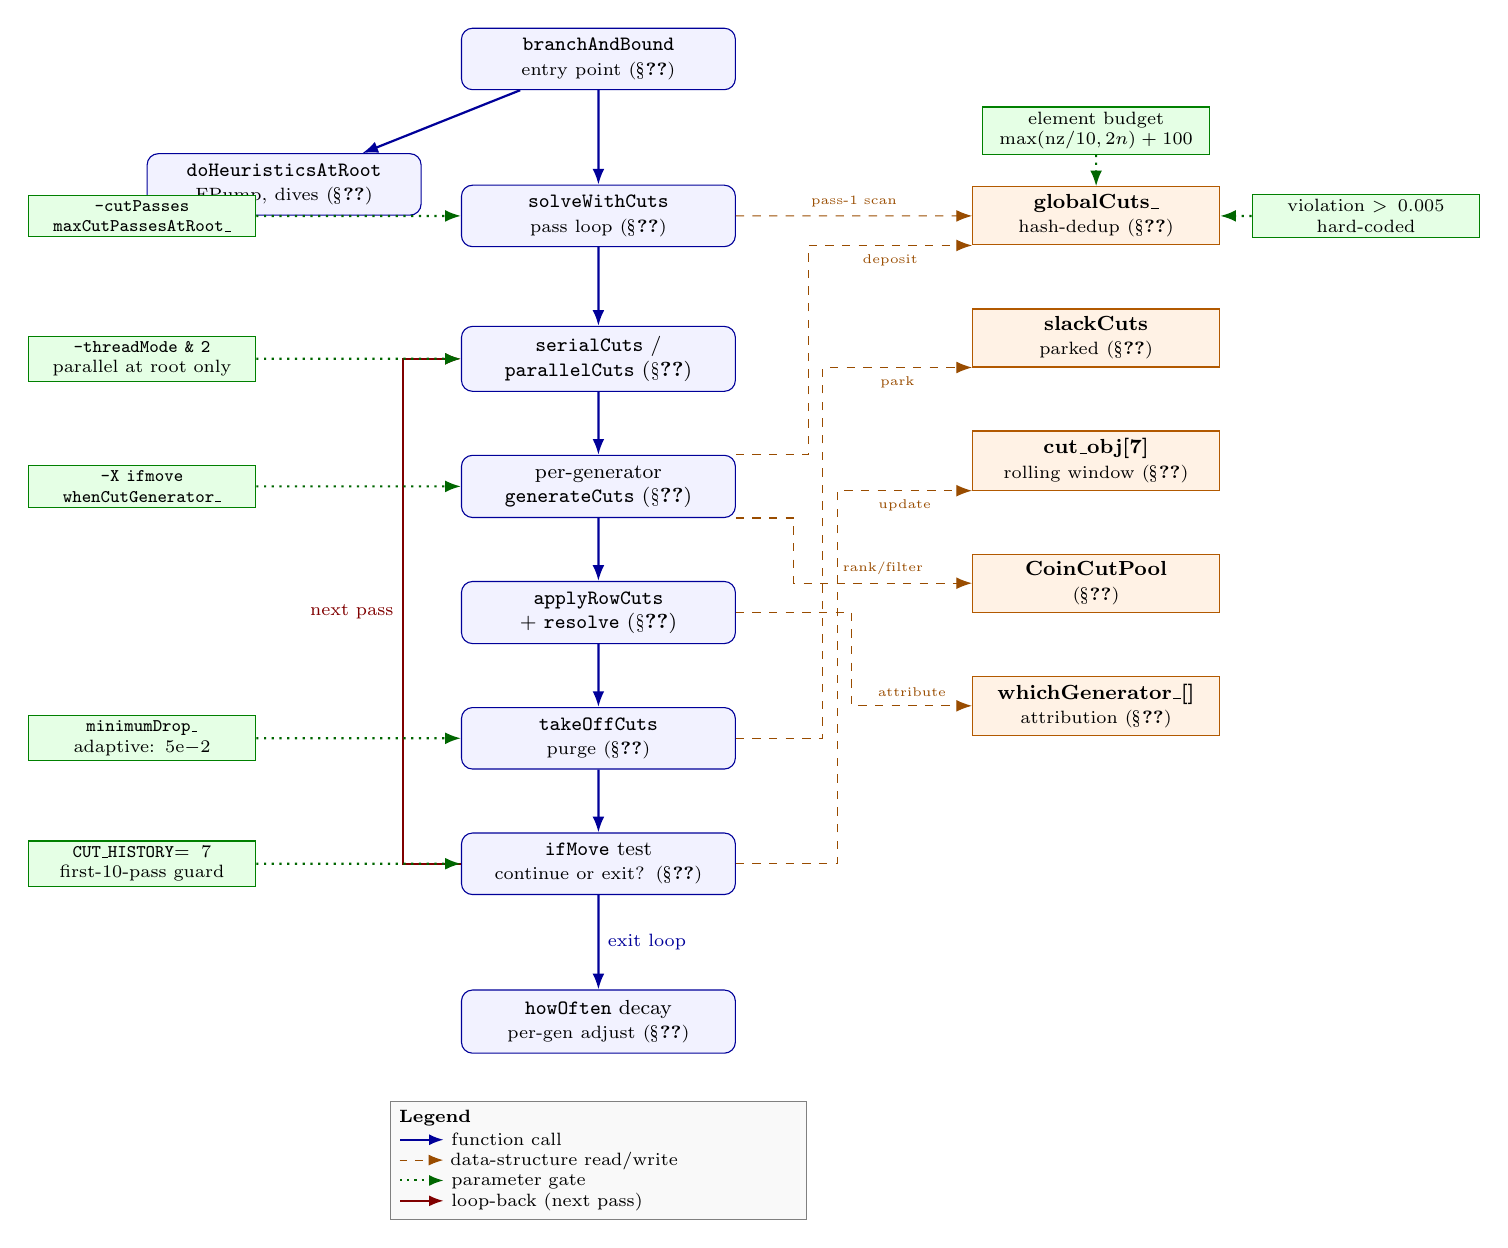
\begin{tikzpicture}[scale=0.92, every node/.style={scale=0.92},
  font=\footnotesize,
  node distance=6mm and 8mm,
  method/.style={rectangle, draw=blue!60!black, fill=blue!5,
                 rounded corners, align=center, inner sep=4pt,
                 minimum height=7mm, text width=35mm},
  ds/.style    ={rectangle, draw=orange!70!black, fill=orange!10,
                 align=center, inner sep=3pt, minimum height=6mm,
                 text width=32mm},
  param/.style ={rectangle, draw=green!50!black, fill=green!10,
                 align=center, inner sep=2pt, minimum height=5mm,
                 text width=30mm, font=\scriptsize},
  call/.style  ={-{Latex[length=2mm]}, thick, blue!60!black},
  rw/.style    ={-{Latex[length=2mm]}, dashed, orange!60!black},
  gate/.style  ={-{Latex[length=2mm]}, dotted, green!40!black,
                 thick},
  loop/.style  ={-{Latex[length=2mm]}, thick, red!50!black},
]

% === LEFT: Method flow (vertical) ===
\node[method] (bab) {\texttt{branchAndBound}\\\scriptsize entry point (\S\ref{sec:bab})};

\node[method, below left=8mm and 5mm of bab] (heur)
  {\texttt{doHeuristicsAtRoot}\\\scriptsize FPump, dives (\S\ref{sec:heurroot})};

\node[method, below=12mm of bab] (swc)
  {\texttt{solveWithCuts}\\\scriptsize pass loop (\S\ref{sec:rootloop})};

\node[method, below=10mm of swc] (serial)
  {\texttt{serialCuts} /\\\texttt{parallelCuts} (\S\ref{sec:parallel})};

\node[method, below=8mm of serial] (gen)
  {per-generator\\\texttt{generateCuts} (\S\ref{sec:howoften})};

\node[method, below=8mm of gen] (apply)
  {\texttt{applyRowCuts}\\$+$ \texttt{resolve} (\S\ref{sec:applyresolve})};

\node[method, below=8mm of apply] (takeoff)
  {\texttt{takeOffCuts}\\\scriptsize purge (\S\ref{sec:takeoff})};

\node[method, below=8mm of takeoff] (ifmove)
  {\texttt{ifMove} test\\\scriptsize continue or exit? (\S\ref{sec:ifmove})};

\node[method, below=12mm of ifmove] (decay)
  {\texttt{howOften} decay\\\scriptsize per-gen adjust (\S\ref{sec:howoften})};

% === RIGHT: Data structures ===
\node[ds, right=30mm of swc] (gpool)
  {\textbf{globalCuts\_}\\\scriptsize hash-dedup (\S\ref{sec:cutpool})};

\node[ds, below=8mm of gpool] (slack)
  {\textbf{slackCuts}\\\scriptsize parked (\S\ref{sec:takeoff})};

\node[ds, below=8mm of slack] (history)
  {\textbf{cut\_obj[7]}\\\scriptsize rolling window (\S\ref{sec:ifmove})};

\node[ds, below=8mm of history] (ccp)
  {\textbf{CoinCutPool}\\\scriptsize (\S\ref{sec:cutpool-vs-coincutpool})};

\node[ds, below=8mm of ccp] (which)
  {\textbf{whichGenerator\_[]}\\\scriptsize attribution (\S\ref{sec:treedata})};

% === FAR LEFT: Parameters ===
\node[param, left=26mm of swc] (pCutPass)
  {\texttt{-cutPasses}\\\texttt{maxCutPassesAtRoot\_}};

\node[param, left=26mm of serial] (pThread)
  {\texttt{-threadMode \& 2}\\\scriptsize parallel at root only};

\node[param, left=26mm of gen] (pHowOften)
  {\texttt{-X ifmove}\\\texttt{whenCutGenerator\_}};

\node[param, left=26mm of takeoff] (pMinDrop)
  {\texttt{minimumDrop\_}\\\scriptsize adaptive: $5\mathrm{e}{-2}$};

\node[param, left=26mm of ifmove] (pHistory)
  {\texttt{CUT\_HISTORY}$=7$\\\scriptsize first-10-pass guard};

% === Calls ===
\draw[call] (bab) -- (swc);
\draw[call] (bab) -- (heur);
\draw[call] (swc) -- (serial);
\draw[call] (serial) -- (gen);
\draw[call] (gen) -- (apply);
\draw[call] (apply) -- (takeoff);
\draw[call] (takeoff) -- (ifmove);
\draw[call] (ifmove) -- (decay)
  node[midway, right, font=\scriptsize]{exit loop};

% Loop-back arrow
\draw[loop] (ifmove.west) -- +(-8mm,0)
  |- node[near start, left, font=\scriptsize]{next pass}
  (serial.west);

% === Data-structure reads/writes ===
\draw[rw] (swc.east) -- node[above, font=\tiny]{pass-1 scan} (gpool.west);
\draw[rw] (gen.north east) -- ++(10mm,0) |- (gpool.south west)
  node[near end, below, font=\tiny]{deposit};
\draw[rw] (gen.south east) -- ++(8mm,0) |- (ccp.west)
  node[near end, above, font=\tiny]{rank/filter};
\draw[rw] (takeoff.east) -- ++(12mm,0) |- (slack.south west)
  node[near end, below, font=\tiny]{park};
\draw[rw] (ifmove.east) -- ++(14mm,0) |- (history.south west)
  node[near end, below, font=\tiny]{update};
\draw[rw] (apply.east) -- ++(16mm,0) |- (which.west)
  node[near end, above, font=\tiny]{attribute};

% === Gates (params -> methods) ===
\draw[gate] (pCutPass.east) -- (swc.west);
\draw[gate] (pThread.east) -- (serial.west);
\draw[gate] (pHowOften.east) -- (gen.west);
\draw[gate] (pMinDrop.east) -- (takeoff.west);
\draw[gate] (pHistory.east) -- (ifmove.west);

% === Hardcoded constants near globalCuts ===
\node[param, above=4mm of gpool] (pBudget)
  {element budget\\\scriptsize $\max(\text{nz}/10,2n)+100$};
\node[param, right=4mm of gpool] (pViol)
  {violation $> 0.005$\\\scriptsize hard-coded};
\draw[gate] (pBudget.south) -- (gpool.north);
\draw[gate] (pViol.west) -- (gpool.east);

% === Legend ===
\node[draw=gray, fill=gray!5, align=left, font=\scriptsize,
      below=6mm of decay, anchor=north, text width=55mm]
  (legend) {%
   \textbf{Legend}\\[1pt]
   \tikz\draw[call] (0,0) -- (6mm,0); function call\\
   \tikz\draw[rw]   (0,0) -- (6mm,0); data-structure read/write\\
   \tikz\draw[gate] (0,0) -- (6mm,0); parameter gate\\
   \tikz\draw[loop] (0,0) -- (6mm,0); loop-back (next pass)};

\end{tikzpicture}
\end{center}

\subsection*{Diagram 2: Tree-node cut lifecycle}

\begin{center}
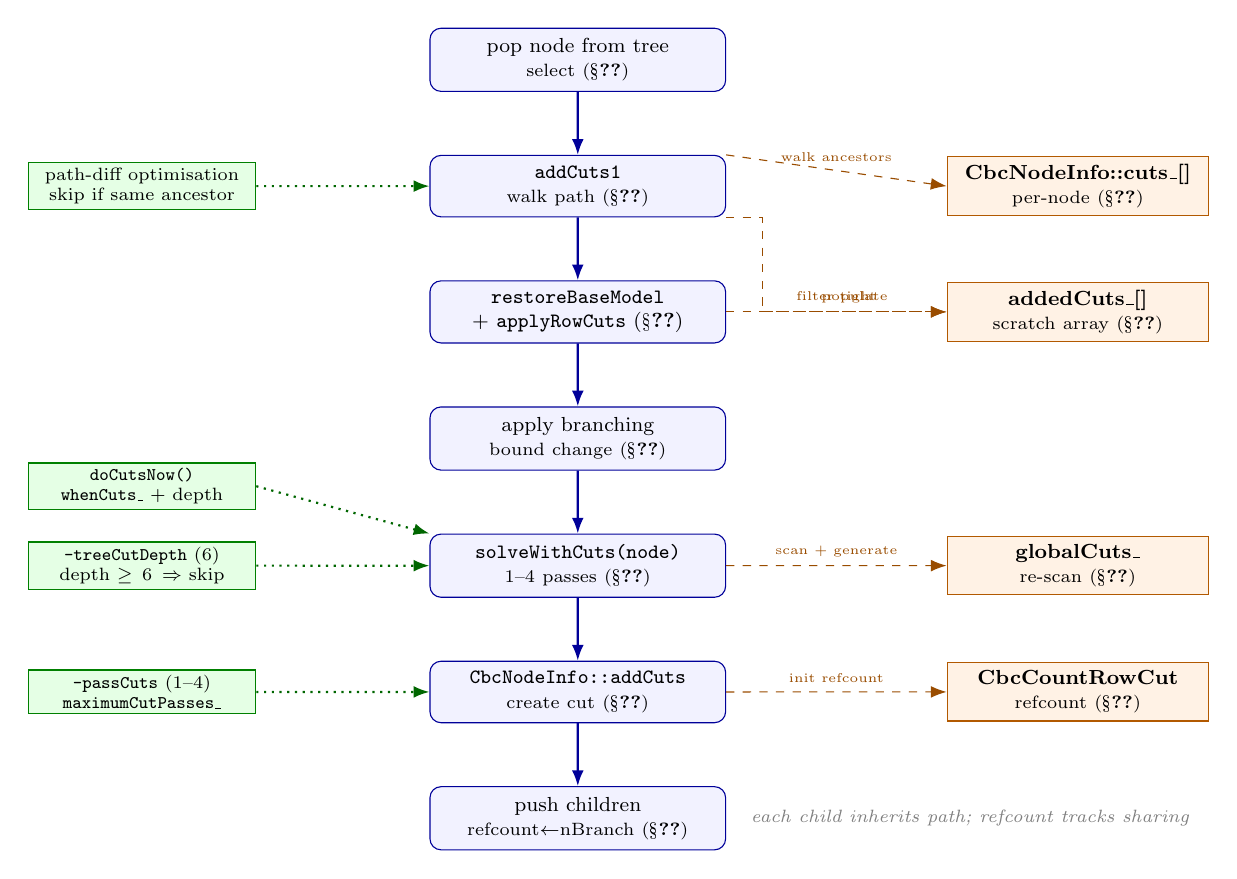
\begin{tikzpicture}[scale=0.92, every node/.style={scale=0.92},
  font=\footnotesize,
  node distance=6mm and 8mm,
  method/.style={rectangle, draw=blue!60!black, fill=blue!5,
                 rounded corners, align=center, inner sep=4pt,
                 minimum height=7mm, text width=38mm},
  ds/.style    ={rectangle, draw=orange!70!black, fill=orange!10,
                 align=center, inner sep=3pt, minimum height=6mm,
                 text width=34mm},
  param/.style ={rectangle, draw=green!50!black, fill=green!10,
                 align=center, inner sep=2pt, minimum height=5mm,
                 text width=30mm, font=\scriptsize},
  call/.style  ={-{Latex[length=2mm]}, thick, blue!60!black},
  rw/.style    ={-{Latex[length=2mm]}, dashed, orange!60!black},
  gate/.style  ={-{Latex[length=2mm]}, dotted, green!40!black,
                 thick},
]

% === Method flow ===
\node[method] (pop) {pop node from tree\\\scriptsize select (\S\ref{sec:nodeselect})};

\node[method, below=8mm of pop] (addcuts)
  {\texttt{addCuts1}\\\scriptsize walk path (\S\ref{sec:restore})};

\node[method, below=8mm of addcuts] (restore)
  {\texttt{restoreBaseModel}\\$+$ \texttt{applyRowCuts} (\S\ref{sec:restore})};

\node[method, below=8mm of restore] (branch)
  {apply branching\\\scriptsize bound change (\S\ref{sec:nodeselect})};

\node[method, below=8mm of branch] (swcnode)
  {\texttt{solveWithCuts(node)}\\\scriptsize 1--4 passes (\S\ref{sec:treeparams})};

\node[method, below=8mm of swcnode] (store)
  {\texttt{CbcNodeInfo::addCuts}\\\scriptsize create cut (\S\ref{sec:treedata})};

\node[method, below=8mm of store] (push)
  {push children\\\scriptsize refcount$\gets$nBranch (\S\ref{sec:nodeselect})};

% === Data structures (right) ===
\node[ds, right=28mm of addcuts] (nodeinfo)
  {\textbf{CbcNodeInfo::cuts\_[]}\\\scriptsize per-node (\S\ref{sec:treedata})};

\node[ds, right=28mm of restore] (added)
  {\textbf{addedCuts\_[]}\\\scriptsize scratch array (\S\ref{sec:treedata})};

\node[ds, right=28mm of swcnode] (gpool)
  {\textbf{globalCuts\_}\\\scriptsize re-scan (\S\ref{sec:cutpool})};

\node[ds, right=28mm of store] (refcount)
  {\textbf{CbcCountRowCut}\\\scriptsize refcount (\S\ref{sec:treedata})};

% === Parameters (left) ===
\node[param, left=22mm of addcuts] (pSame)
  {path-diff optimisation\\\scriptsize skip if same ancestor};

\node[param, left=22mm of swcnode] (pTreeCD)
  {\texttt{-treeCutDepth} (6)\\\scriptsize depth $\ge 6 \Rightarrow$ skip};

\node[param, above=4mm of pTreeCD] (pDocuts)
  {\texttt{doCutsNow()}\\\texttt{whenCuts\_} + depth};

\node[param, left=22mm of store] (pPassCuts)
  {\texttt{-passCuts} (1--4)\\\texttt{maximumCutPasses\_}};

% === Calls ===
\draw[call] (pop) -- (addcuts);
\draw[call] (addcuts) -- (restore);
\draw[call] (restore) -- (branch);
\draw[call] (branch) -- (swcnode);
\draw[call] (swcnode) -- (store);
\draw[call] (store) -- (push);

% === Data-structure connections ===
\draw[rw] (addcuts.north east) -- (nodeinfo.west)
  node[midway, above, font=\tiny]{walk ancestors};
\draw[rw] (addcuts.south east) -- ++(5mm,0) |- (added.west)
  node[near end, above, font=\tiny]{populate};
\draw[rw] (restore.east) -- (added.west |- restore.east)
  node[midway, above, font=\tiny]{filter tight};
\draw[rw] (swcnode.east) -- (gpool.west)
  node[midway, above, font=\tiny]{scan + generate};
\draw[rw] (store.east) -- (refcount.west)
  node[midway, above, font=\tiny]{init refcount};

% === Gates ===
\draw[gate] (pSame.east) -- (addcuts.west);
\draw[gate] (pTreeCD.east) -- (swcnode.west);
\draw[gate] (pDocuts.east) -- (swcnode.north west);
\draw[gate] (pPassCuts.east) -- (store.west);

% === Annotations ===
\node[font=\scriptsize\itshape, text=gray, right=2mm of push]
  {each child inherits path; refcount tracks sharing};

\end{tikzpicture}
\end{center}

\paragraph{How to read the diagrams.}
\textbf{Diagram~1} (root) shows the pass loop inside
\texttt{solveWithCuts}: generators fire in batch, cuts are applied
and resolved, \texttt{takeOffCuts} purges non-binding ones, and the
\texttt{ifMove} test decides whether to loop or exit.  Parameters
on the left gate each step; data structures on the right are
written/read at the indicated points.  The red loop-back arrow shows
the per-pass iteration.

\textbf{Diagram~2} (tree) shows the lifecycle at each non-root
node: the LP is reconstructed wholesale from the ancestor path
(\texttt{addCuts1} $\to$ \texttt{restoreBaseModel}), branching is
applied, then \texttt{solveWithCuts} runs 1--4 passes (gated by
\texttt{treeCutDepth} and \texttt{doCutsNow}).  New cuts become
\texttt{CbcCountRowCut} objects owned by the node's
\texttt{CbcNodeInfo}, with refcount initialised to the number of
child branches.

\section{Tree-side cut data structures and lifecycle}
\label{sec:treedata}

Understanding how cuts survive beyond the root and are
reconstructed at each tree node requires knowledge of five
interacting data structures.

\subsection*{1. \texttt{addedCuts\_} --- the per-node scratch array}

\begin{lstlisting}
// CbcModel.hpp:3146
CbcCountRowCut **addedCuts_;
int maximumNumberCuts_;   // allocated capacity
int currentNumberCuts_;   // entries currently valid
\end{lstlisting}

\texttt{addedCuts\_} is a \textbf{temporary array rebuilt each time
a node is selected from the tree}.  It collects pointers to every
\texttt{CbcCountRowCut} on the root$\to$node path.  It does
\emph{not} own the cuts --- the actual owners are the
\texttt{CbcNodeInfo} objects (see below).

\textbf{Population:} \texttt{addCuts1(node, lastws)} at
\texttt{CbcModel.cpp:7969} walks the tree path, calling
\texttt{applyToModel()} on each ancestor; each call appends that
ancestor's \texttt{cuts\_[]} entries into
\texttt{addedCuts\_[offset..]}.

\textbf{Filtering:} after population, code at line~8169 classifies
each entry as \emph{tight} (non-basic in the warm-start) or
\emph{loose} (basic).  Loose entries are set to \texttt{NULL} (and
reference-counted down).  Only tight cuts are installed in the LP.

\textbf{Cleanup during cut generation:} \texttt{takeOffCuts}
(line~11341) decrements and possibly frees entries that become
slack after a resolve.

\textbf{Fathoming:} when a node is pruned by bound
(line~8326--8337), \emph{all} entries are decremented by
\texttt{numberBranchesLeft} and freed if refcount reaches zero.

\subsection*{2. \texttt{CbcCountRowCut} --- reference-counted cut}

\begin{lstlisting}
// CbcCountRowCut.hpp
class CbcCountRowCut : public OsiRowCut {
  CbcNodeInfo *owner_;           // back-pointer to owning node
  int          ownerCut_;        // index in owner's cuts_[]
  int          numberPointingToThis_;  // reference count
  int          whichCutGenerator_;
};
\end{lstlisting}

\textbf{Reference counting protocol:}
\begin{itemize}[leftmargin=*]
  \item \textbf{Creation:} initialised to the number of child
        branches that will inherit it (typically~2).
  \item \textbf{Decrement sites:}
    (a)~node fathomed by bound (all its inherited cuts lose
        \texttt{numberBranchesLeft} refs),
    (b)~\texttt{takeOffCuts} removes a slack ancestor cut ($-1$),
    (c)~tree cleanup on node deletion ($-$numberLeft).
  \item \textbf{At zero:} the destructor calls
        \texttt{owner\_->deleteCut(ownerCut\_)} to null the slot in
        the owning \texttt{CbcNodeInfo}'s \texttt{cuts\_[]} array.
\end{itemize}

\texttt{canDropCut()} (line~97--112 of \texttt{CbcCountRowCut.cpp})
returns \texttt{false} for cuts with
\texttt{effectiveness()$=$COIN\_DBL\_MAX} (never droppable) and for
\texttt{effectiveness()$>1\mathrm{e}10$} cuts that are currently
tight.

\subsection*{3. \texttt{CbcNodeInfo} --- per-node persistent storage}

\begin{lstlisting}
// CbcNodeInfo.hpp
class CbcNodeInfo {
  CbcCountRowCut **cuts_;   // cuts generated AT this node
  int numberCuts_;           // length of cuts_[]
  int numberRows_;           // rows before these cuts
  CbcNodeInfo *parent_;      // chain to root
};
\end{lstlisting}

Each \texttt{CbcNodeInfo} stores \emph{only} the cuts generated at
that specific node.  The full cut set is implicitly the union along
the root$\to$node path, reconstructed lazily by
\texttt{addCuts1()}.

\texttt{CbcNodeInfo::addCuts(OsiCuts\&, numberToBranch,
numberPointingToThis)} at \texttt{CbcNodeInfo.cpp:326} allocates
\texttt{CbcCountRowCut} objects, sets \texttt{owner\_=this} and
the initial refcount to \texttt{numberToBranch}.  It is called
after \texttt{solveWithCuts} returns new cuts (line~16737).

\texttt{CbcPartialNodeInfo} (the common case) additionally stores a
\emph{basis diff} and bound changes applied at this node.

\subsection*{4. \texttt{whichGenerator\_[]} --- cut attribution}

\begin{lstlisting}
// CbcModel.hpp:3427
int *whichGenerator_;   // sized maximumWhich_ (initial 1000)
\end{lstlisting}

Maps active cut positions (from
\texttt{numberRowsAtContinuous\_}) to generators.  Encoding:

\begin{tabular}{ll}
\toprule
Value & Meaning\\
\midrule
\texttt{i + 10000} & root/global cut from generator~$i$\\
\texttt{i + 20000} & tree-generated cut from generator~$i$\\
\texttt{20099} & cut from globalCuts\_ pool (unattributed)\\
\texttt{20098} & stored/reinstated global cut\\
\bottomrule
\end{tabular}

Used by the post-loop decay logic to count how many cuts each
generator has active, then adjust \texttt{howOften} adaptively.

\subsection*{5. Row layout in the solver}

At any node, the LP row structure is:

\begin{lstlisting}
[0 .. numberRowsAtContinuous_-1]                = original LP rows
[numberRowsAtContinuous_ .. + numberOldActiveCuts_-1] = ancestor cuts
[.. + numberNewCuts_-1]                         = this node's cuts
\end{lstlisting}

\texttt{numberOldActiveCuts\_} = ancestor cuts still tight after
\texttt{addCuts1} filtering.  \texttt{numberNewCuts\_} = cuts
generated in \texttt{solveWithCuts} at this node.

\section{Node cut restoration: the wholesale rebuild}
\label{sec:restore}

Unlike some MIP solvers that incrementally add/remove cuts when
moving between nodes, MIPster uses a \textbf{wholesale rebuild}:

\begin{enumerate}[leftmargin=*]
  \item \textbf{Walk root$\to$node.}
        \texttt{addCuts1()} walks the parent chain via
        \texttt{walkback\_[]}, collecting all \texttt{CbcNodeInfo*}
        and summing their cut counts.

  \item \textbf{Apply path.}
        Traverses \texttt{walkback\_[]} from root to node.  Each
        \texttt{CbcPartialNodeInfo::applyToModel()} applies:
        (a)~basis diff, (b)~bound changes from branching,
        (c)~copies its \texttt{cuts\_[]} pointers into
        \texttt{addedCuts\_[]}.

  \item \textbf{Filter tight vs.\ loose.}
        Each cut's warm-start basis status is inspected:
        non-basic $\Rightarrow$ tight (keep), basic $\Rightarrow$
        loose (drop, decrement refcount).  Exception:
        \texttt{effectiveness()$>1\mathrm{e}10$} cuts that
        \texttt{canDropCut()} refuses.

  \item \textbf{Strip + reinstall.}
\begin{lstlisting}
solver_->restoreBaseModel(numberRowsAtContinuous_);
solver_->applyRowCuts(numberToAdd, addCuts);
solver_->setWarmStart(lastws);
\end{lstlisting}

  \item \textbf{Optimisation: path diff.}
        Lines~8016--8068 compare the new path with
        \texttt{lastNodeInfo\_[]} (previous node's path).  If paths
        share ancestors, only the divergent suffix needs processing.
        If identical (\texttt{sameProblem=true}), the whole rebuild
        is skipped.
\end{enumerate}

\textbf{Why wholesale, not incremental?}  The warm-start basis and
the tight/loose classification change across nodes.  Re-evaluating
every ancestor cut against the new basis is cheaper than tracking
individual insertions/deletions --- particularly since
\texttt{OsiClp::restoreBaseModel} is an O(1) pointer reset (it
stores a cached matrix at the continuous).

\section{\texttt{fullScan} and periodic generator re-evaluation}
\label{sec:fullscan}

The \texttt{fullScan} variable in \texttt{serialCuts}
(\texttt{CbcModel.cpp:9112--9118}) controls whether all generators
run or only frequent ones:

\begin{lstlisting}
int fullScan = 0;
if ((numberNodes_ % SCANCUTS) == 0 || (specialOptions_ & 256) != 0) {
  fullScan = 1;
  if (!numberNodes_ || (specialOptions_ & 256) != 0)
    fullScan = 2;
}
\end{lstlisting}

\begin{tabular}{ll}
\toprule
\texttt{fullScan} & Meaning\\
\midrule
0 & Normal: only generators with active \texttt{howOften} run; those
    with \texttt{switchOff} are skipped.\\
1 & Periodic (every \texttt{SCANCUTS}$=$1000 nodes): all generators
    fire to re-assess which should remain active.\\
2 & Root (\texttt{numberNodes\_$=$0}) or new-solution trigger
    (\texttt{specialOptions\_\&256}): most aggressive scan; drives
    the \texttt{willBeCutsInTree} decision.\\
\bottomrule
\end{tabular}

The companion variable \texttt{switchOff} (line~11003) is:
\begin{lstlisting}
int switchOff = (!doCutsNow(1) && !fullScan) ? 1 : 0;
\end{lstlisting}
When \texttt{switchOff$=$1}, generators with default frequency are
silently skipped --- this is how the depth-based
\texttt{doCutsNow()} gating actually suppresses generators in the
tree without modifying their \texttt{howOften}.

\section{\texttt{moreSpecialOptions\_} and \texttt{specialOptions\_}
         cut-related bits}
\label{sec:specbits}

\subsection*{\texttt{moreSpecialOptions\_} (CbcModel.hpp:3209)}

\begin{longtable}{p{2.2cm}p{1.5cm}p{10cm}}
\toprule
\textbf{Bits} & \textbf{Mask} & \textbf{Effect on cuts}\\
\midrule
\endhead
11--12 & \texttt{>>11 \&3} & \texttt{experimentBreak}:
  0=old style early-exit, 1=new style, 2=no break if zero cuts
  first time, 3=as~2 but last drop must be $>0.1\cdot$min.\\
13 & 8192 & \texttt{increaseDrop}: ramp up
  \texttt{minimumDrop\_} across passes (bail out faster).\\
16 & 65536 & No cuts during preprocessing.\\
20 & 1048576 & Resolve LP \emph{before} cut generation starts
  (reduce sum of infeasibilities).\\
21 & 2097152 & Resolve LP \emph{after} cuts at root.\\
\bottomrule
\end{longtable}

\subsection*{\texttt{specialOptions\_} (CbcModel.hpp:3178)}

\begin{longtable}{p{2.2cm}p{1.8cm}p{9.7cm}}
\toprule
\textbf{Bit} & \textbf{Value} & \textbf{Effect on cuts}\\
\midrule
\endhead
0 & 1 & \texttt{debugCuts} mode (OsiRowCutDebugger active).\\
8 & 256 & New solution found $\Rightarrow$ trigger full generator
  scan at next node (\texttt{fullScan$=$2}).\\
11 & 2048 & Small sub-B\&B: skip \texttt{treeCutDepth\_} check.\\
12 & 4096 & ``Funny cuts, do slow way'' (affects
  \texttt{restoreBaseModel} path).\\
13 & 8192 & Same as 4096 in alternative code paths.\\
23 & 8388608 & Leave cuts in solver after solve (don't strip).\\
\bottomrule
\end{longtable}

\section{Complete parameter catalog}
\label{sec:catalog}

\subsection*{A. CLI parameters (tunable)}

\begin{longtable}{p{4.0cm}p{2.0cm}p{8.5cm}}
\toprule
\textbf{Parameter} & \textbf{Default} & \textbf{Purpose}\\
\midrule
\endhead
\texttt{-cutPasses}          & 100       & Root pass cap (overridden adaptively
  to 50/100/$-100$ based on column count).\\
\texttt{-passCuts}           & 1         & Per-tree-node pass cap (maps to
  \texttt{maximumCutPasses\_}; solver uses~4 adaptively).\\
\texttt{-treeCutDepth}       & 6         & Hard depth cutoff for cuts in tree.\\
\texttt{-cutDepth}           & $-1$      & Per-generator depth modulus
  (\texttt{depthCutGenerator\_}).\\
\texttt{-cuts}               & on        & Master \texttt{whenCuts\_} control
  (on/root/ifmove/forceOn/off).\\
\texttt{-slowcutpasses}      & 10        & Cap on calls to slow generators
  (RedSplit, LandP).\\
\texttt{-cutLength}          & $-1$      & Gomory cut density cap.\\
\texttt{-conflictCuts}       & on        & Dive conflict-cut harvest.\\
\texttt{-multipleRootSolvers}& off       & Race LP/cut configs at root.\\
\texttt{-threadMode}         & 0         & Bit~2: parallel root cuts.\\
\texttt{-cliqueCuts}         & ifmove    & BKClique generator mode.\\
\texttt{-flowCoverCuts}      & ifmove    & Flow cover generator mode.\\
\texttt{-gomoryCuts}         & ifmove    & Gomory generator mode.\\
\texttt{-knapsackCuts}       & ifmove    & Knapsack cover generator mode.\\
\texttt{-mixedIntegerRoundingCuts} & ifmove & MIR generator mode.\\
\texttt{-oddwheelCuts}       & off       & Odd-wheel generator mode.\\
\texttt{-probingCuts}        & ifmove    & Probing generator mode.\\
\texttt{-twoMirCuts}         & ifmove    & TwoMIR generator mode.\\
\texttt{-zeroHalfCuts}       & ifmove    & ZeroHalf generator mode.\\
\texttt{-reduceAndSplitCuts} & off       & RedSplit generator mode.\\
\texttt{-reduce2AndSplitCuts}& ifmove    & RedSplit2 generator mode.\\
\texttt{-GMICuts}            & off       & GMI generator mode.\\
\texttt{-liftAndProjectCuts} & off       & LandP generator mode.\\
\texttt{-lagomoryCuts}       & off       & Lagomory generator mode.\\
\texttt{-latwomirCuts}       & off       & LaTwoMIR generator mode.\\
\texttt{-residualCapacityCuts}& off      & ResidualCapacity generator mode.\\
\texttt{-pathAggrCuts}       & root      & Path aggregation generator mode.\\
\texttt{-zeroHalfSparseThreshold}& 8000  & ZeroHalf: switch to sparse graph.\\
\texttt{-zeroHalfRowMaxPairCount}& 150000& ZeroHalf: skip dense rows.\\
\texttt{-cutRankingMetric}      & fitness& Scoring formula at all 3 ranking
  sites: \texttt{violation} (raw LP violation) or \texttt{fitness}
  ($(viol/activeCols)\cdot10^5 + (1/(\Delta_C+1))\cdot10^3$).\\
\texttt{-cutPoolFilter}         & on    & Enable per-round
  best-per-variable filter (\texttt{filterCutsByBestPerVar}).\\
\texttt{-cutPoolFilterMinCuts}  & 50    & Minimum row cuts per round
  to activate the filter; rounds with fewer cuts are unfiltered.\\
\texttt{-globalCutMinViolation} & 0.005 & Minimum violation for a
  global-pool cut to be re-admitted to the LP.\\
\bottomrule
\end{longtable}

\subsection*{B. Per-generator internal defaults
             (\texttt{installCutGenerators})}

\begin{longtable}{p{2.5cm}p{5.5cm}p{1.8cm}p{3.0cm}}
\toprule
\textbf{Generator} & \textbf{Key limits set} & \textbf{Accuracy} &
  \textbf{\texttt{switchOffIfLessThan}}\\
\midrule
\endhead
Probing & \texttt{maxPass=1, maxProbe=123, maxLook=10/20,
  maxElements=200/300, rowCuts=$-3$} & 5 & 0\\
Gomory  & \texttt{limitAtRoot=1000, limit=50, awayAtRoot=0.005}
  & 3 & 0\\
Knapsack & (no special limits) & 1 & 0\\
MIR/Flow & (default params) & 2 & 0\\
PathAggr & (no special limits) & 2 & 0\\
TwoMIR  & \texttt{maxElements=250, awayAtRoot=0.005, away=0.01}
  & 4 & \textbf{1} (disabled pass~0 if 0 cuts)\\
Clique  & (CoinCutPool-based selection inside) & 0 & 0\\
OddWheel& (CoinCutPool-based selection inside) & 0 & 0\\
ZeroHalf& sparse threshold 8000, pair-count 150000 & 5 &
  \textbf{2} (disabled pass~0 if $<$2 cuts)\\
RedSplit/LandP & \texttt{maximumTries=slowcutpasses (10)} & 5 &
  0 (uses \texttt{maximumTries\_} instead)\\
\bottomrule
\end{longtable}

\subsection*{C. Hardcoded constants (candidates for CLI promotion)}

\begin{longtable}{p{4.0cm}p{2.5cm}p{2.5cm}p{5.5cm}}
\toprule
\textbf{Constant} & \textbf{Value} & \textbf{Source} &
\textbf{What it controls}\\
\midrule
\endhead
Global-pool element budget & $\max(\text{nz}/10,2n)+100$ &
  CbcModel.cpp:9342 & Maximum NZ the LP can grow per global-pool
  injection.\\
\texttt{CUT\_HISTORY} & 7 & CbcModel.cpp:8549 & Rolling-window
  length for ifMove early-exit.\\
First-pass guard & $\ge 10$ & CbcModel.cpp:9669 & Suppress early
  termination for first 10 passes.\\
Slack re-admit cutoff & $100\,\tau_{\text{prim}}$ &
  CbcModel.cpp:11109 & Tolerance for re-injecting parked cuts.\\
Small-model threshold & $\le 500$ & CbcModel.cpp:18899 & Triggers
  simpler \texttt{doCutsNow} branch.\\
\texttt{TRY\_IDEA1} depth gate & $=10$ & CbcModel.cpp:18934 &
  Where \texttt{allowForTopOfTree=3} fires.\\
\texttt{SCANCUTS} & 1000 & CbcCutGenerator.hpp:608 & Nodes
  between full generator scans.\\
Dive conflict cap & 128 & CbcRootHeuristicSchedule:26 & Top-$K$
  for dive conflict cuts.\\
Density abandon thresholds & 1e-5 obj, 20\% nz &
  CbcModel.cpp:$\sim$10270 & Disables tree cuts if root cuts
  didn't help but bloated the LP.\\
\texttt{drop[12]} table & $\{1,2,3,10,\dots,1000\}$ &
  CbcModel.cpp:9670 & Per-depth bonus on ifMove
  early-termination.\\
\texttt{effectiveness $> 1\mathrm{e}10$} & $10^{10}$ &
  CbcModel.cpp:8179 & Threshold for ``always keep'' cuts
  (below COIN\_DBL\_MAX).\\
\bottomrule
\end{longtable}

\section{Putting it together}

A typical root iteration looks like this:

\begin{enumerate}[leftmargin=*]
  \item LP solve $\Rightarrow$ fractional solution $x^\ast$.
  \item Pre-cut heuristics may produce an incumbent.
  \item Pass~1 of \texttt{solveWithCuts}:
    \begin{itemize}
      \item Scan \texttt{globalCuts\_} for violations of $x^\ast$,
            sort by violation, add up to a matrix-element budget.
      \item Run all enabled generators (serial, or parallel if
            \texttt{threadMode\_\&2}).
      \item Apply, resolve.
      \item \texttt{takeOffCuts}: drop slack cuts whose
            effectiveness is finite.
      \item Update \texttt{cut\_obj} history; check \texttt{badObj}
            / \texttt{goodDrop}.
    \end{itemize}
  \item Pass~$k\!>\!1$: as above plus a primal-heuristic block on
        the new $x^\ast$ before the cut generation.
  \item Loop ends when (a) the pass cap is hit, or (b) the
        \texttt{ifMove} test (\S\ref{sec:ifmove}) fires while no
        generator is in \texttt{mustCallAgain} mode.
  \item Post-loop adjustment: every generator's \texttt{howOften} is
        rewritten based on its yield; ineffective ones drop to
        $-99$.
  \item Branch.  Inside the tree, \texttt{solveWithCuts} runs again
        with \texttt{maximumCutPasses\_} (default 4 in MIPster), no
        global-pool re-scan beyond pass~1, no parallel cuts, and
        deeper-than-\texttt{treeCutDepth\_} nodes skip cuts
        entirely.
\end{enumerate}

A typical \textbf{tree node} iteration:

\begin{enumerate}[leftmargin=*]
  \item Pop node from tree.  Call \texttt{addCuts(node, lastws)}:
    \begin{itemize}
      \item \texttt{addCuts1}: walk root$\to$node, rebuild
            \texttt{addedCuts\_[]}, classify tight vs.\ loose.
      \item \texttt{restoreBaseModel} + \texttt{applyRowCuts}
            (tight only) + \texttt{setWarmStart}.
    \end{itemize}
  \item Apply branching decision (bound change).
  \item LP resolve.  If infeasible or fathomed by bound, prune
        (decrement refcounts on inherited cuts, done).
  \item \texttt{solveWithCuts(cuts, maximumCutPasses\_, node)}:
    \begin{itemize}
      \item \texttt{treeCutDepth\_} gate: depth $\ge 6
            \Rightarrow$ skip.
      \item \texttt{doCutsNow()} gate: depth/modular check.
      \item If allowed: run \texttt{serialCuts}, apply, resolve,
            \texttt{takeOffCuts} --- typically only 1 pass.
    \end{itemize}
  \item Store results: \texttt{CbcNodeInfo::addCuts()} creates
        \texttt{CbcCountRowCut} objects for new cuts with initial
        refcount = number of child branches.
  \item Push child nodes to tree.
\end{enumerate}

\section*{File index}

\begin{tabular}{ll}
\toprule
File & Role\\
\midrule
\texttt{src/CbcModel.cpp}             & root/tree orchestration, cut loop, take-off, pool scan,
                                         addCuts1\\
\texttt{src/CbcModel.hpp}             & \texttt{maximumCutPasses[AtRoot]\_}, \texttt{globalCuts\_},
                                         \texttt{addedCuts\_}, \texttt{whichGenerator\_}\\
\texttt{src/CbcCutGenerator.cpp/hpp}  & per-generator gating, switches bitfield,
                                         \texttt{SCANCUTS}\\
\texttt{src/CbcCountRowCut.cpp/hpp}   & \texttt{CbcRowCuts} pool, dedup; \texttt{CbcCountRowCut}
                                         refcounting\\
\texttt{src/CbcNodeInfo.hpp}           & per-node cut storage (\texttt{cuts\_[]}, \texttt{numberCuts\_}),
                                         tree walk helpers\\
\texttt{src/CbcPartialNodeInfo.cpp}    & \texttt{applyToModel}: basis diff + bounds +
                                         cut population\\
\texttt{src/CbcThread.cpp}            & \texttt{parallelCuts}, threading mode bits\\
\texttt{src/CbcSolver.cpp}            & adaptive defaults, generator/heuristic registration\\
\texttt{src/CbcSolverCutSetup.cpp}    & \texttt{installCutGenerators}: per-generator limits\\
\texttt{src/CbcParameters.cpp}        & CLI parameter setup, defaults\\
\texttt{src/CbcTree.cpp}              & tree cleanup, refcount decrement on deleted nodes\\
\bottomrule
\end{tabular}

\end{document}
